% id: 140-18
% book: 베이직쎈 미적분1 · 09 정적분의 활용
% section: 개념 57 두 곡선 사이의 넓이
% passage: 다음 그림에서 색칠한 부분의 넓이를 구하시오.
% figure: tikz:fig-140-18
% answer: 
% answer_source: 
% variant_level: 0 (원본 전사)
% 이 파일은 build.mjs 가 items.json 에서 만든다. 고칠 때는 items.json 을 고친다.
\smash{\raisebox{1.5mm}{\dmkichul{베이직쎈 미적분1 140쪽 18번}}}
\noindent\begin{minipage}[t]{0.58\linewidth}\vspace{0pt}\raggedright \end{minipage}\hfill\begin{minipage}[t]{0.4\linewidth}\vspace{0pt}\centering \resizebox{\ifdim\width>\linewidth\linewidth\else\width\fi}{!}{% 140-18(140쪽) — 두 곡선 $y=x^2+2x$ 와 $y=-x^2$ 로 둘러싸인 색칠한 부분($x=-1$ 에서 $x=0$ 까지). 스캔 화질이 낮아 TikZ 로 다시 그림.
% 원문에 있는 것만 옮긴다: 두 포물선 · 색칠 · $x=-1$ 의 안내 점선 · 라벨 y=x^2+2x, y=-x^2, -2, -1, O, x, y. 원문에 없는 눈금·넓이 값은 적지 않는다.
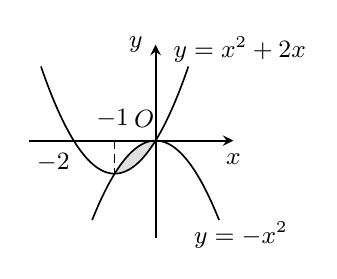
\begin{tikzpicture}[x=0.52cm, y=0.42cm, line width=0.6pt]
  \fill[gray!25] plot[domain=-1:0, samples=60, smooth] (\x, {-(\x)*(\x)}) -- plot[domain=0:-1, samples=60, smooth] (\x, {(\x)*(\x)+2*(\x)}) -- cycle;
  \draw[->, >=stealth, line width=0.7pt] (-3.1,0) -- (1.9,0) node[below=1pt, font=\small] {$x$};
  \draw[->, >=stealth, line width=0.7pt] (0,-2.95) -- (0,2.9) node[left=1pt, font=\small] {$y$};
  \draw[densely dashed, line width=0.4pt] (-1,0) -- (-1,-1);
  \draw[domain=-2.8:0.8, samples=100, smooth] plot (\x, {(\x)*(\x)+2*(\x)});
  \draw[domain=-1.55:1.55, samples=100, smooth] plot (\x, {-(\x)*(\x)});
  \node[below=1pt, font=\small] at (-2.5,0) {$-2$};
  \node[above=1pt, font=\small] at (-1.05,0) {$-1$};
  \node[above=1pt, font=\small] at (-0.28,0) {$\pt{O}$};
  \node[anchor=west, inner sep=1pt, font=\small] at (0.35,2.75) {$y=x^2+2x$};
  \node[anchor=west, inner sep=1pt, font=\small] at (0.85,-2.85) {$y=-x^2$};
\end{tikzpicture}
}\end{minipage}\par
\dmhint{$\displaystyle\int_{-1}^{0} \{-x^2-(\blank[3.6em])\}\mkern3mu dx$\\ $\displaystyle =\int_{-1}^{0} (-2x^2-\blank[1.1em])\mkern3mu dx$\\ $\displaystyle =\Big[-\dfrac{2}{3}x^3-\blank[1.1em]\Big]_{-1}^{0}$\\ $=\blank$}
